\documentclass[12pt,a4paper]{article}
% \usepackage[latin1]{inputenc}
\usepackage[english]{babel}
\usepackage{amsmath}
\usepackage{amsfonts}
\usepackage{amssymb}
\usepackage{svg}
\usepackage{url}
\usepackage{hyperref}

\author{
  Katrien Laenen\\
  \and
  Gust Verbruggen\\
  \and
  Ward Schodts
}
\title{Knowledge \& the web: exercise session 6}
\begin{document}
\maketitle
In this report we discuss which algorithms we tried to find a good classification model that predicts if a passenger of the Titanic will survive or not.
We use the data from \texttt{titanic\_train.csv} to train our model and perform cross-validation for performance assessment. The models used are a \textbf{rule set} and a \textbf{decision tree}.  The rest of this document is structured as follows. First we describe the preprocessing steps used in order to prepare the data for better classification. Next, we describe the learning process for both models. Finally, we compare results for both learning techniques, based on the cross-validation results. 

\section{Preprocessing}
In order to achieve better classification, we preprocess the data. This is done in two phases: feature selection to only preserve relevant features and feature engineering in the form of a discretisation step.

\paragraph{Feature selection} Features that we do not think are relevant are \texttt{Name}, \texttt{Ticket}, \texttt{PassengerId}, \texttt{Embarked} and \texttt{Cabin}. They are removed.

\paragraph{Discretisation} The two numerical values are discretised in accordance to some criterium. The \texttt{Age} feature into five age classes: child ($<$ 9 years), teen (10 to 15 years), young (15 to 24 years), adult (25 to 59 years) and elderly ($>$ 59 years). To discretise \texttt{Fare}, we take a look at a histogram plot, as seen in Figure~\ref{fig:histfare}. There are a lot more low fares. The three leftmost bars get their own bin. The chosen discretisation is: 0-10, 10-20, 20-30, 30-100 and 100+.

\begin{figure}[htbp]
	\centering
	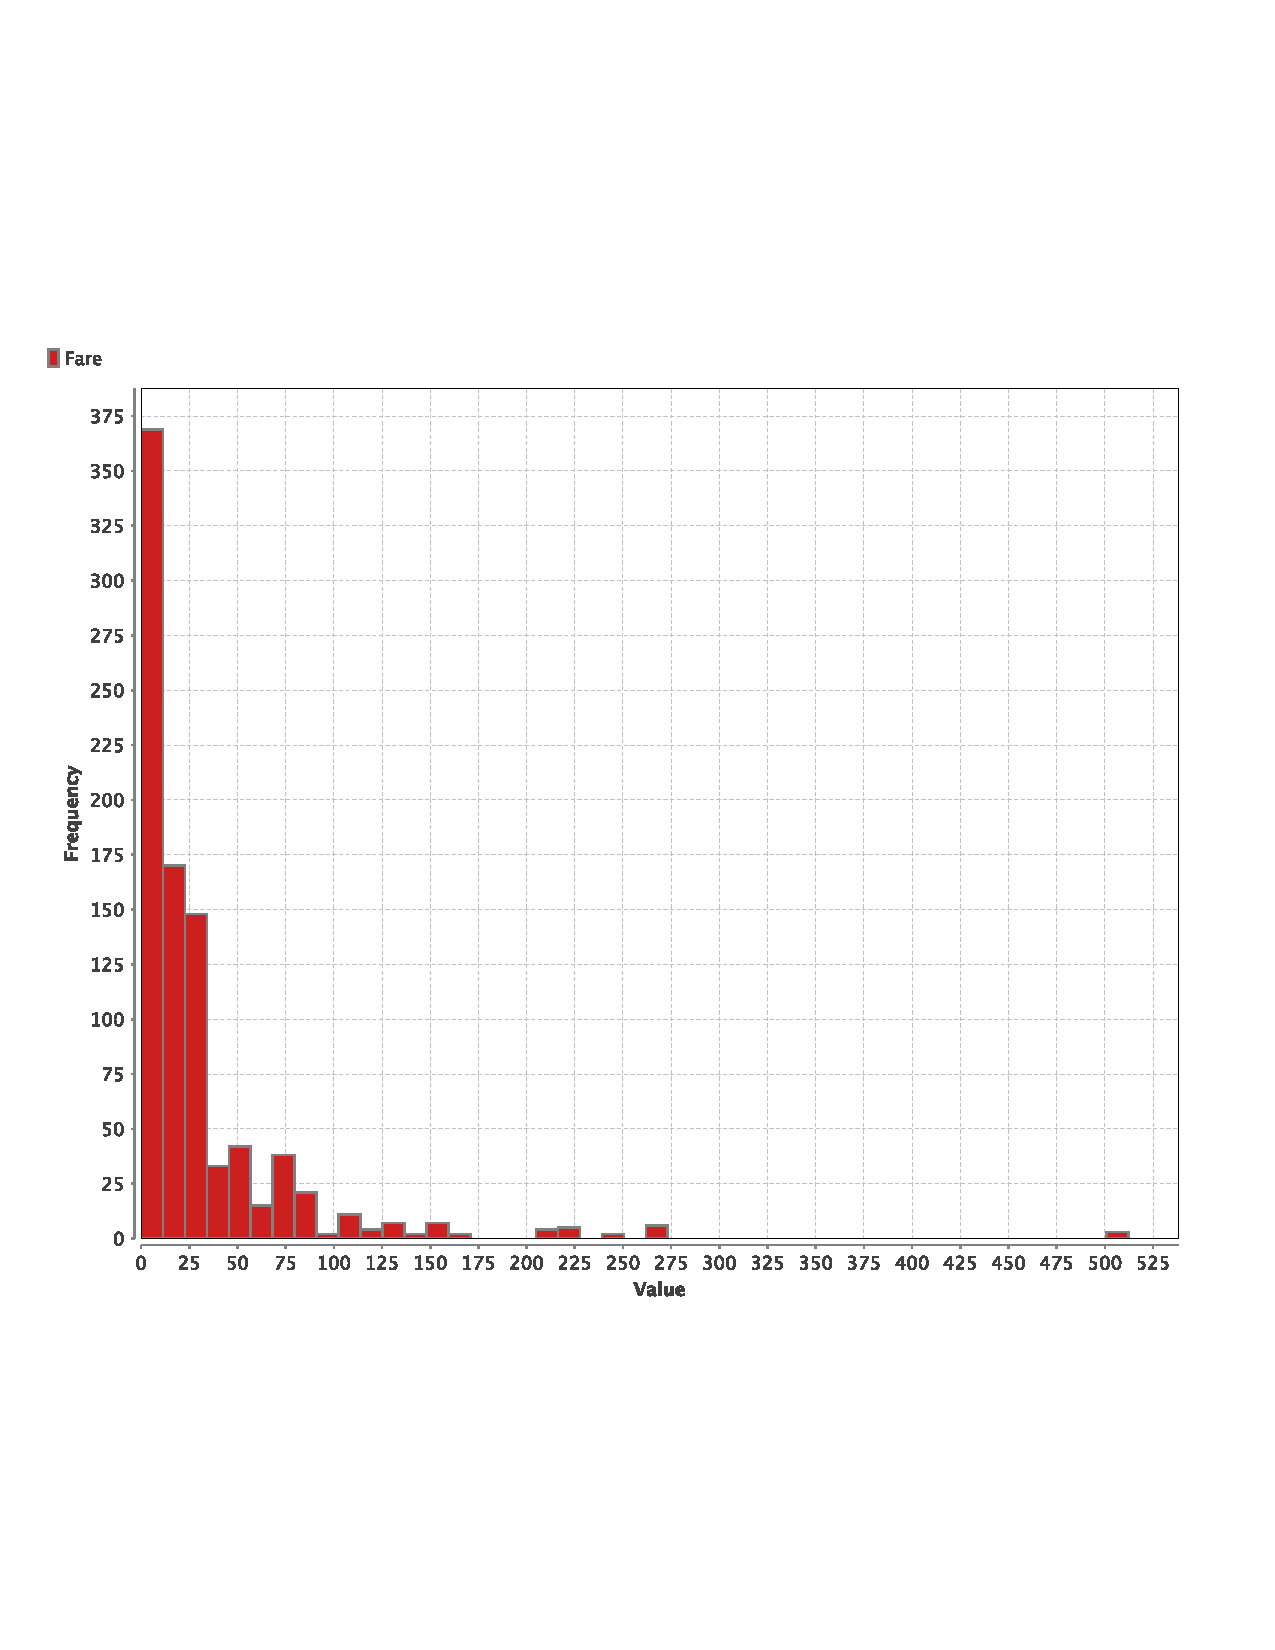
\includegraphics[width = .7\textwidth]{fare_histogram.pdf}
	\caption{Histogram for the \texttt{Fare} feature}
	\label{fig:histfare}
\end{figure}


\section{Rule learning}
One thing we tried was to learn classification rules from the training data.
Rule learning algorithms come with different options for several aspects of the algorithms. In the exercise session we experimented with two of these.\\
First, for choosing the conditions of a classification rule, there are two options: one is to add to the rule the condition which increases the accuracy the most, another is to add to the rule the condition which increases the information gain the most.\\
The accuracy criterion option resulted in the following rule set:
\begin{itemize}

\item if Parch > 5.500 then 0  (1 / 0)
\item if Fare = >10 and Sex = male then 0  (170 / 25)
\item if Sex = female then 1  (63 / 197)
\item else 0  (171 / 61)

\end{itemize}
%which is correct for 539 out of 688 training examples.
The information gain criterion option resulted in this rule set:
\begin{itemize}

\item if Sex = male and Fare = >10 then 0  (170 / 25)
\item if Sex = female then 1  (64 / 197)
\item if Fare = 10-20 and Parch ≤ 0.500 then 0  (66 / 7)
\item else 0  (111 / 54)

\end{itemize}
%which is correct for 544 out of 694 training examples.
A second aspect of rule learning is the desired pureness, which is the minimum ratio of the major class in a covered subset in order to consider the subset pure. The standard value for this is 0.9. We experimented with this value set to 0.8 and 1.
For the desired pureness set to 0.8 and the accuracy criterion we got the following rule set:
\begin{itemize}

\item if Parch > 5.500 then 0  (1 / 0)
\item if Fare = >10 then 0  (189 / 47)
\item if Sex = female then 1  (44 / 175)
\item else 0  (171 / 61)

\end{itemize}
%which is correct for 536 out of 688 training examples.
This rule set is very similar to the rule set obtained with the accuracy criterion option and desired pureness of 0.9. The only difference is that in the second rule the \textit{Sex = male} condition now disappeared from the condition part. 
For the desired pureness set to 0.8 and the information gain criterion we got the following rule set:
\begin{itemize}

\item if Sex = male then 0  (360 / 93)
\item else 1  (57 / 177)

\end{itemize}
%which is correct for 537 out of 687 training examples.
When comparing this rule set with the rule set obtained for the information gain criterion with the desired pureness set to 0.9, we see that this rule set is a great simplification of the other.
For the desired pureness set to 1 and the accuracy criterion we got exactly the same rule set as when setting the desired pureness to 0.9 for that criterion. The same happened for the desired pureness set to 1 and the information gain criterion, which also resulted in the same rule set as when setting the pureness to 0.9 and keeping the information criterion.\\
Next to the criterion and desired pureness, there are three other parameters for rule learning: sample ratio (which specifies the sample ratio of training data used for growing and pruning), minimal prune benefit (which specifies the minimum amount of benefit which must be exceeded over unpruned benefit in order to be pruned) and use local random seed (which indicates if a local random seed should be used for randomization). We did not experiment with these parameters, but kept the standard values for these, which were 0.9, 0.25 and no respectively.\\
\\
From these results we can clearly see that Sex, Fare and Parch are features which are important for this task. That Sex and Fare were important features was to be expected. When the Titanic collided with an iceberg, women and children and people of the higher ranks were evacuated first. This is reflected in the data as we see that women and people which payed a higher fare are more likely to have survived. That the number of parents and children is also an important feature can be explained as follows. People in need want to stay close to their loved ones at all costs. But how larger a group, how more difficult it was to get on a lifeboat together. Also, little children and old people need much more assistence to even reach a lifeboat. As such, how more children and parents someone had aboard, how less likely that person was to survive.

\section{Decision trees}

%\begin{figure}[htbp]
%  \centering
%  \includesvg[width = 0.7\textwidth]{decisiontreetitanic}
%  \caption{Decision tree with maximal depth of 3}
%\end{figure}

\section{?}


\end{document}
